\chapter{Problematyka zagadnienia}
\label{ch:problematyka}

%---------------------------------------------------------------------------
\section{Charakterystyka choroby Parkinsona}
\label{sec:charakterystykaPD}

Choroba Parkinsona (PD) jest zwyrodnieniowym schorzeniem mózgu związanym z objawami motorycznymi (spowolnienie ruchowe,
drżenie, sztywność, zaburzenia chodu i równowagi) oraz szeroką gamą powikłań niemotorycznych (zaburzenia poznawcze,
zaburzenia psychiczne, zaburzenia snu oraz ból i inne zaburzenia sensoryczne).
Objawy zwykle zaczynają się stopniowo i nasilają z czasem.
Ich postęp powoduje wysoki stopień niepełnosprawności i konieczność opieki.
U wielu osób z PD w trakcie trwania choroby mogą również rozwinąć się zmiany psychiczne i behawioralne, problemy ze snem,
depresja, problemy z pamięcią i zmęczenie.

\begin{figure}[htbp]
	\centering
	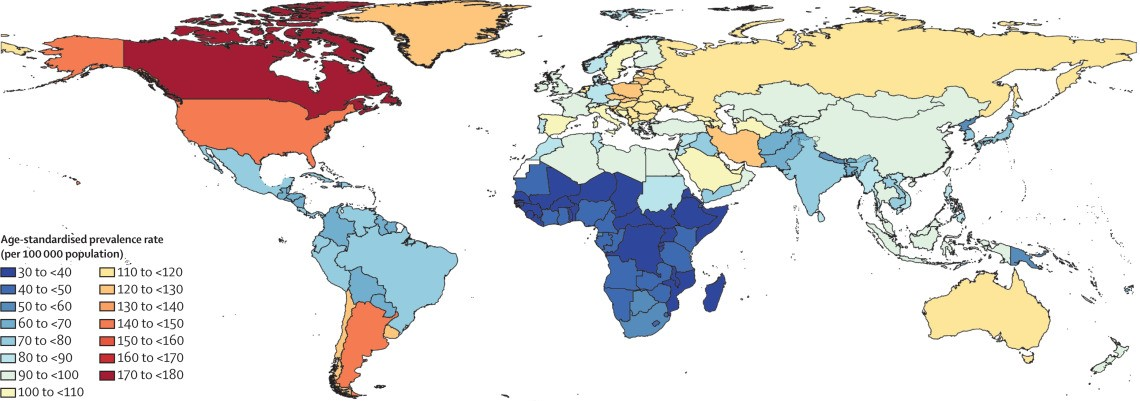
\includegraphics[width=0.9\textwidth]{./img/map}
	\caption{Choroba Parkinsona na świecie \cite{global_PD}}
    \label{fig:PD_map}
\end{figure}

Według raportu Światowej Organizacji Zdrowia\cite{WHO} w skali globalnej niepełnosprawność i zgony z powodu PD
rosną szybciej niż w przypadku jakichkolwiek innych zaburzeń neurologicznych.
Częstość występowania PD podwoiła się w ciągu ostatnich 25 lat.
Globalne szacunki w 2019 roku wykazały ponad 8,5 miliona osób z PD.
Obecne szacunki sugerują, że w 2019 roku PD spowodowała 5,8 miliona lat życia z niepełnosprawnością, co
stanowi wzrost o 81\% od 2000 roku, i spowodowała 329 000 zgonów, co stanowi wzrost o ponad 100\% od 2000 roku.

W Polsce z chorobą Parkinsona zmaga się około 100 tys. pacjentów, z czego około 20\% jest już w stadium zaawansowanym
według informacji przekazywanych przez Fundację Chorób Mózgu.
Ponadto co roku w naszym kraju wykrywanych jest ok. 8 tys. nowych zachorowań.
Nowe zachorowania nadal skorelowane są z wiekiem, średnia wieku chorych wynosi 60 lat, niestety wzrasta odsetek chorych wśród osób młodych (nawet w wieku 20 lat).

Przyczyna PD nie jest znana, ale uważa się, że powstaje w wyniku złożonej interakcji pomiędzy czynnikami genetycznymi i
narażeniem na czynniki środowiskowe, takie jak pestycydy, rozpuszczalniki i zanieczyszczenia powietrza.
Niektóre przypadki PD wydają się być dziedziczne, a kilka przypadków można przypisać określonym wariantom genetycznym.
Chociaż uważa się, że genetyka odgrywa rolę w chorobie Parkinsona, w większości przypadków choroba nie występuje rodzinnie\cite{National_Institute_on_Aging_2022}.

\begin{figure}[htbp]
	\centering
	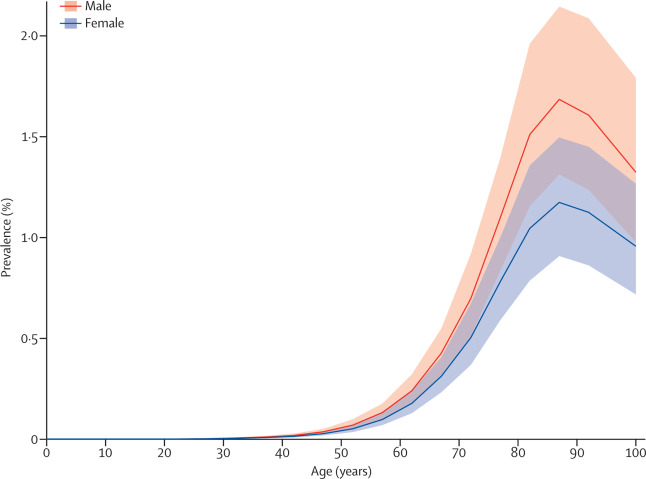
\includegraphics[width=0.6\textwidth]{./img/PD_prevalence}
	\caption{Rozpowszechnienie choroby Parkinsona w zależności od wieku \cite{global_PD}}
    \label{fig:PD_prevalance}
\end{figure}

Chociaż każdy może być narażony na ryzyko rozwoju choroby Parkinsona, badania naukowe sugerują,
że choroba ta dotyka więcej mężczyzn niż kobiet.
Statystyki pokazują, że ryzyko zachorowania rośnie wraz z wiekiem, chociaż choroba może dotyczyć także młodszych osób.
U większości osób z PD po raz pierwszy choroba rozwija się po 60 roku życia, około 5\% do 10\% doświadcza jej początku przed 50 rokiem życia.
Postacie choroby Parkinsona o wczesnym początku są często, choć nie zawsze, dziedziczne i niektóre formy zostały powiązane z
określonymi zmianami w genach\cite{National_Institute_on_Aging_2022}.

%---------------------------------------------------------------------------

\subsection{Objawy choroby}
\label{subsec:objawy}

Najbardziej widoczne oznaki i objawy choroby Parkinsona pojawiają się, gdy komórki nerwowe w zwojach podstawy mózgu,
obszarze mózgu kontrolującym ruch, ulegają uszkodzeniu i/lub obumierają.
Zwykle te komórki nerwowe lub neurony wytwarzają dopaminę.
Kiedy neurony obumierają lub ulegają uszkodzeniu, wytwarzają mniej dopaminy, co powoduje problemy z poruszaniem się
związane z chorobą.
Na ten moment nie wiadomo co powoduje śmierć neuronów.
Zanikają również zakończenia nerwowe, które wytwarzają norepinefrynę, główny przekaźnik chemiczny
współczulnego układu nerwowego, który kontroluje wiele funkcji organizmu, takich jak tętno i ciśnienie krwi.
Utrata norepinefryny może pomóc wyjaśnić niektóre cechy choroby Parkinsona związane z brakiem ruchu, takie jak zmęczenie,
nieregularne ciśnienie krwi, zmniejszony ruch pokarmu w przewodzie pokarmowym i nagły spadek ciśnienia krwi, gdy osoba wstaje z pozycji siedzącej lub leżącej.


Do czterech głównych objawów choroby Parkinsona zalicza się:
\begin{itemize}[itemsep=0.5pt]
	\item Drżenie rąk, ramion, nóg, szczęki lub głowy
	\item Sztywność mięśni, gdy mięśnie pozostają skurczone przez długi czas
	\item Powolność ruchu
	\item Zaburzenia równowagi i koordynacji, czasami prowadzące do upadków
\end{itemize}


Pozostałe objawy mogą obejmować:
\begin{itemize}[itemsep=0.5pt]
	\item Depresja i inne zmiany emocjonalne
	\item Trudności w połykaniu, żuciu i mówieniu
	\item Problemy z układem moczowym lub zaparcia
	\item Problemy skórne
\end{itemize}

Objawy choroby Parkinsona i tempo progresji różnią się u poszczególnych osób.
Początkowo są subtelne i pojawiają się stopniowo.
Często zaczynają się po jednej stronie ciała lub nawet w jednej kończynie.
W miarę postępu choroby ostatecznie dotyka ona obu stron, jednak objawy mogą być bardziej nasilone po jednej stronie niż po drugiej.
Wiele osób z chorobą Parkinsona zauważa, że przed wystąpieniem sztywności i drżenia miały problemy ze snem, zaparcia, utratę węchu oraz zespół niespokojnych nóg.
Należy pamiętać, że niektóre z tych objawów mogą również wystąpić podczas normalnego starzenia się \cite{National_Institute_on_Aging_2022}.

Chociaż postęp choroby Parkinsona jest zwykle powolny, ostatecznie może to wpłynąć na codzienne czynności danej osoby. Czynności takie jak praca, zajmowanie się domem i udział w zajęciach towarzyskich z przyjaciółmi mogą stać się wyzwaniem. Doświadczanie tych zmian może być trudne, ale grupy wsparcia mogą pomóc ludziom sobie z tym poradzić. Grupy te mogą dostarczać informacji, porad i łączy z zasobami dla osób żyjących z chorobą Parkinsona, ich rodzin i opiekunów.


%---------------------------------------------------------------------------

\subsection{Etapy choroby}
\label{subsec:etapy}

Tu będę opierać się na tym\cite{Szurek_2018} i na tym\cite{Wieczorek_2013} i na tym\cite{Kuryłowicz_2019}

Wielu lekarzy, którzy diagnozują to zaburzenie mózgu, polega na skali oceny Hoehna i Yahra, aby sklasyfikować nasilenie objawów.
Skala jest podzielona na pięć etapów w zależności od postępu choroby.
Pięć etapów pomaga lekarzom ocenić, jak daleko zaawansowana jest choroba.

W praktyce klinicznej często dodaje się stopnie pośrednie (1,5, 2,5, 3,5 i 4,5), które spełniają kryteria stopnia niższego, ale obecne są (niestale lub w niewielkim nasileniu) objawy kwalifikujące do stopnia wyższego.

\begin{itemize}[itemsep=0.5pt]
	\item Etap 0.0: Brak objawów choroby
	\item Etap 1.0: Łagodny: objawy parkinsonowskie tylko po jednej stronie ciała
	\item Etap 1.5: Objawy jednostronne i osiowe.
	\item Etap 2.0: Objawy po obu stronach ciała (zwykle z przewagą jednej z nich), bez zaburzeń równowagi
	\item Etap 2.5: Łagodne obustronne zajęcie z powrotem do zdrowia w teście retropulsacji (pull).
	\item Etap 3.0: Zaburzenia równowagi, łagodna lub średnio zaawansowana choroba, niezależność w zakresie samoobsługi
	\item Etap 4.0: Ciężka niepełnosprawność, jednak chory jest w stanie poruszać się i utrzymywać postawę stojącą bez pomocy innych osób
	\item Etap 5.0: Chory wymaga wózka inwalidzkiego lub jest całkowicie unieruchomiony w łóżku
\end{itemize}

[https://www.parkinson.org/understanding-parkinsons/what-is-parkinsons/stages]
Jedną z krytyki skali Hoehna i Yahra jest fakt, że skupia się ona wyłącznie na kwestiach związanych z ruchem i wynikającymi z niego problemami. Jednak inne objawy są związane z PD, takie jak różne formy zmian poznawczych i upośledzenia, w tym początek stanów, takich jak zaburzenia zachowania podczas snu REM.

Z tego powodu niektórzy lekarze wybierają alternatywę, zunifikowaną skalę oceny choroby Parkinsona MDS. Skala ta składa się z pięćdziesięciu kompleksowych pytań służących do analizy objawów motorycznych i niemotorycznych w celu uzyskania szerszego spojrzenia na trudności pacjenta.
Ich odkrycia mogą pomóc w ocenie upośledzeń funkcji poznawczych, które utrudniają codzienne zadania, obok problemów z poruszaniem się, w oferowaniu skuteczniejszych form leczenia.
Chociaż jest bardziej złożony, zapewnia lekarzom dokładniejszy wgląd w specyficzne upośledzenia i potrzeby danej osoby. Dysponując większą wiedzą i danymi, lekarze uzyskują pełniejszy obraz stanu psychicznego i fizycznego danej osoby, a nie tylko jej zdolności motorycznych.

Do wczesnych objawów choroby Parkinsona zalicza się [https://www.parkinson.org/understanding-parkinsons/what-is-parkinsons/stages]:
\begin{itemize}[itemsep=0.5pt]
	\item drżenie palców, kciuków, dłoni lub podbródka
	\item drobne lub stłoczone pismo odręczne
	\item utrata węchu
	\item problemy ze snem
	\item problemy z poruszaniem się lub chodzeniem
	\item zaparcie
	\item miekki lub niski głos
	\item zamaskowan twarz
	\item zawroty głowy i omdlenia
	\item pochylanie się lub garbienie się
\end{itemize}

%---------------------------------------------------------------------------

\subsection{Terapia osób chorych}
\label{subsec:terapia}
Obecnie brak jest kuracji na chorobę Parkinsona, dlatego terapia skupia się na przywracaniu pacjentom zdolności funkcjonowania
lub, w przypadkach zaawansowanych, na poprawie jakości życia.
Zgodnie z aktualnym standardem medycznym, w terapii wykorzystuje się różnorodne metody, w tym leczenie farmakologiczne, głęboką stymulację mózgu oraz rehabilitację \cite{National_Institute_on_Aging_2022}.

Leczenie farmakologiczne choroby Parkinsona opiera się na zwiększeniu poziomu dopaminy w mózgu, co wpływa na kontrolę objawów
ruchowych i niezwiązanych z ruchem. Główną terapią jest lewodopa, która jest przetwarzana przez komórki nerwowe w dopaminę.
Leczenie lewodopą często łączy się z karbidopą, która zmniejsza skutki uboczne i ilość potrzebnej lewodopy.
Stosuje się też inne terapie farmakologiczne o różnych zasadach działania m.in. pobudzające produkcję dopaminy,
zwiększające ilość dopaminy poprzez spowolnienie jej rozkładu, redukujące ruchy mimowolne czy zmniejszające drżenie i sztywność mięśni.

W przypadku pacjentów, u których leczenie farmakologiczne nie przynosi oczekiwanych efektów, może być rozważana Głęboka Stymulacja Mózgu (DBS).
W tym procederze chirurgicznym lekarz implantuje elektrody w określone obszary mózgu, łącząc je z małym urządzeniem elektrycznym umieszczonym w klatce piersiowej.
Poprzez bezbolesne stymulowanie konkretnych obszarów mózgu kontrolujących ruch, DBS może pomóc w zmniejszeniu wielu objawów związanych z ruchem,
takich jak drżenie, spowolnienie ruchu i sztywność.

Kluczową rolę w leczeniu odgrywa rehabilitacja neurologiczna, rozpoczynając się już od momentu postawienia diagnozy.
Jej wsparcie jest nieocenione w łagodzeniu zaburzeń chodu, głosu, drżenia, sztywności oraz pogorszenia funkcji umysłowych.
Wśród różnorodnych terapii, znajdują się między innymi:
\begin{itemize}[itemsep=0.1pt]
	\item Zbilansowana Dieta: Odpowiednio zbilansowana dieta odgrywa istotną rolę we wspieraniu ogólnego samopoczucia pacjenta.
	\item Ćwiczenia Fizyczne: Regularne ćwiczenia wzmacniają mięśnie, poprawiają równowagę, elastyczność i koordynację, co może znacząco wpłynąć na jakość życia.
	\item Masaż Terapeutyczny: Masaż terapeutyczny pomaga w redukcji napięcia mięśniowego oraz przynosi ulgę w objawach.
	\item Joga i Tai Chi: Zajęcia z jogi i tai chi wspomagają rozciąganie i elastyczność ciała, co może korzystnie wpłynąć na zdolność ruchową.
	\item Rehabilitacja Foniczna: Specjalistyczna terapia foniczna pomaga w eliminowaniu trudności w mówieniu.
	\item Psychoterapia: Psychoterapia odgrywa istotną rolę w poprawie jakości życia, umożliwiając pacjentom pełne cieszenie się życiem pomimo choroby.
\end{itemize}

Rehabilitacja neurologiczna stanowi nieodzowny element kompleksowego podejścia do zarządzania chorobą Parkinsona, pomagając pacjentom w utrzymaniu jak najwyższej jakości życia.

%---------------------------------------------------------------------------

\section{Metody diagnozowania i monitorowania choroby Parkinsona}
\label{subsec:diagnostyka}

Diagnostyką choroby Parkinsona zajmują się neurolodzy i geriatrzy.
Jej rozwój jest długotrwały, a w początkowych latach klinicznie niemal niewidoczny, co utrudnia wczesne rozpoznanie.
Subtelne objawy często są uważane za skutek starzenia się lub błędnie diagnozowane jako inne zaburzenia neurologiczne.
Kluczowym elementem w tym stadium jest dokładny wywiad, badanie fizykalne oraz identyfikacja objawów przez lekarza.
Następnie diagnoza jest rozwijana poprzez badania laboratoryjne  oraz obrazowe.
Niestety, wyniki tych badań rzadko potwierdzają diagnozę od razu.

Początkowo pacjent zwykle konsultuje się z lekarzem pierwszego kontaktu, który powinien dokonać wstępnej diagnozy i skierować do neurologa.
W tej fazie diagnozy przeprowadza się szczegółowy wywiad, uwzględniający rodzaj, nasilenie oraz okres występowania objawów, a także
obecność chorób neurozwyrodnieniowych w rodzinie.
Neurolog przeprowadza kompleksowe badanie neurologiczne, identyfikując symptomy takie jak sztywność mięśni, ograniczenia w
ruchu (spowolnienie, trudności w poruszaniu się), drżenia spoczynkowe (np. w głowie, palcach rąk) oraz zaburzenia postawy i równowagi
(zgarbienie, niestabilność, upadki). Kolejne badania są wykonywane w celu potwierdzenia lub wykluczenia diagnozy \cite{diagnostyka_Sitek, Loscalzo_2022}.

\renewcommand{\labelenumi}{\alph{enumi})}
\begin{enumerate}
	\item Badania laboratoryjne

Obecnie brak specyficznych badań laboratoryjnych krwi, które potwierdzałyby diagnozę choroby Parkinsona.
Niemniej jednak, takie badania są użyteczne w wykluczaniu innych chorób o podobnym przebiegu.
Wykonuje się podstawowe badania, takie jak morfologia krwi, elektrolity, poziom glukozy, TSH, próby wątrobowe, mocznik, kreatynina oraz poziom witaminy B12.

	\item Badania obrazowe

Badania obrazowe głowy są przeprowadzane w celu wykluczenia innych chorób o podobnych objawach. Pomimo że nie są one szczególnie pomocne w diagnozowaniu choroby Parkinsona, odgrywają ważną rolę w diagnostyce różnicowej. Do tych badań zalicza się tomografię komputerową, ultrasonografię mózgu (USG) oraz rezonans magnetyczny głowy (MRI). Chociaż badania te nie potwierdzają choroby Parkinsona, mogą ujawnić obecność guzów mózgu czy wodogłowia.

Międzynarodowe kryteria rozpoznania choroby Parkinsona nie nakładają obowiązku wykonywania badań obrazowych w celu potwierdzenia diagnozy.
Warto jednak wiedzieć, że dostępne są również zaawansowane techniki obrazowania, takie jak PET (pozytonowa emisyjna tomografia) oraz SPECT (tomografia emisyjna pojedynczego fotonu), które pozwalają na obserwację metabolizmu w układzie pozapiramidowym. Skan DAT (skan transportera dopaminy) jest przykładem SPECT i może być sugerowany przez specjalistę.
Mimo to, ostateczna diagnoza opiera się na objawach oraz wynikach badania neurologicznego. Większość pacjentów nie wymaga skanowania DAT.


	\item Test z lewodopą

Test polega na podaniu pacjentowi podejrzewanemu o chorobę Parkinsona preparatu z lewodopą.
Jeśli następuje poprawa po zażyciu, istnieje wysokie prawdopodobieństwo, że pacjent rzeczywiście cierpi na chorobę Parkinsona.
W przypadku braku poprawy, konieczne może być dalsze rozszerzenie diagnostyki.

	\item Badania genetyczne

Choroba Parkinsona może występować w rodzinach, co skłania do rozważenia diagnostyki genetycznej u pacjenta i jego krewnych.
Badania te są wskazane, gdy lekarz podejrzewa dziedziczne występowanie choroby.
Obecnie zidentyfikowano 12 mutacji genów, które mogą wpływać na ryzyko zachorowania na chorobę Parkinsona.
Należy jednak zaznaczyć, że badania genetyczne są kosztowne.
Proszę, daj znać, czy taka wersja Ci odpowiada, czy może potrzebujesz dalszych zmian.


	\item Badania węchu

Większość osób z chorobą Parkinsona (90\%) doświadcza zaburzeń węchu, manifestujących się hiposomią (osłabienie węchu), także we wczesnym stadium choroby.
Jednak nie obserwuje się tych zaburzeń w przypadku zaniku wieloukładowego i postępującego porażenia nadjądrowego.

	\item Badania neuropsychologiczne i neuropsychiatryczne

Badania te służą identyfikacji zaburzeń poznawczych i emocjonalnych u osób z podejrzeniem choroby Parkinsona.
Psycholodzy i psychiatrzy mają za zadanie diagnozować łagodne zaburzenia poznawcze, otępienie, a także zaburzenia psychotyczne, lękowe, zachowania, kontroli impulsów i depresję.
Proces diagnostyczny jest dostosowany indywidualnie do możliwości pacjenta.
\end{enumerate}

Naukowcy badają test amplifikacji nasion alfa-synukleiny, zdolny do wykrywania choroby Parkinsona przed pojawieniem się objawów.
Test identyfikuje skupiska białka alfa-synukleiny w płynie rdzeniowym, charakterystyczne dla ciał Lewy'ego w mózgu.
Badanie z 2023 roku na ponad 1000 osobach wykazało, że test trafnie rozpoznał chorobę Parkinsona w 87,7\% przypadków.
Wyniki sugerują, że ten test może zmienić podejście do diagnozy, badań i terapii choroby Parkinsona.
Planuje się przyszłe badania oraz nadzieję na mniej inwazyjne metody, takie jak próbki krwi, do przeprowadzania testu \cite{Mayo_Clinic_PD}.

Objawy przypominające chorobę Parkinsona mogą być spowodowane różnymi zaburzeniami, takimi jak zanik wieloukładowy, demencja z ciałami Lewy'ego czy postępujące porażenie nadjądrowe. Te schorzenia są z kolei diagnozowane jako parkinsonizm.

Właściwe odróżnienie między tymi chorobami jest istotne, ponieważ leczenie i podejście terapeutyczne różnią się \cite{National_Institute_on_Aging_2022}.
Badania medyczne oraz reakcja na leczenie farmakologiczne mogą pomóc w ustaleniu dokładnej przyczyny.
Ważne jest, aby uzyskać szybką i dokładną diagnozę.

Choroby o podobnym przebiegu do choroby Parkinsona obejmują m.in. postępujące porażenie nadjądrowe, zanik wieloukładowy, drżenie samoistne, choroby naczyniowe mózgu, otępienie, reumatyzm oraz inne \cite{diagnostyka_Sitek}.
Różnicowanie tych schorzeń jest kluczowe dla właściwego leczenia i zarządzania pacjentem.

Diagnostyka różnicowa choroby Parkinsona obejmuje różne formy parkinsonizmu oraz inne stany neurodegeneracyjne.
Chociaż ostateczną diagnozę można ustalić tylko na podstawie badania mózgu po zgonie, wcześniej zdefiniowane kryteria diagnostyczne pozwalają na dokonanie diagnozy klinicznej.
Przyjęcie ram czasowych (3-10 lat) dla postawienia klinicznie potwierdzonej diagnozy choroby Parkinsona opiera się na empirycznych dowodach.
Wnioski płynące z badania \cite{ROSSI202153} sugerują, że diagnoza klinicznie potwierdzonej choroby Parkinsona może zabierać od kilku miesięcy do kilku lat, zależnie od indywidualnych czynników oraz reakcji na terapię lewodopą.

Chorobę Parkinsona wykluczają także pewne kryteria. Zalicza się do nich:
\begin{itemize}[itemsep=0.5pt]
	\item Historia wielokrotnych urazów głowy,
	\item Przebyte zapalenie mózgu,
	\item Podobne objawy u więcej niż jednej osoby w rodzinie,
	\item Leczenie neuroleptykami w momencie objawów,
	\item Przebyte udary mózgu z nasilonymi objawami parkinsonowskimi,
	\item Długotrwałe ustąpienie objawów,
	\item Objawy po jednej stronie ciała przy chorobie trwającej ponad 3 lata.
\end{itemize}


Pomocnym narzędziem w dianostyce są szeroko stosowane skale oceny choroby Parkinsona.
Stanowią istotne narzędzie w monitorowaniu stanu pacjentów oraz ocenie postępów choroby.
Te strukturalne i skwantyfikowane metody pomagają lekarzom i opiekunom ocenić stopień nasilenia objawów ruchowych,
jak również wpływ choroby na codzienne funkcjonowanie pacjenta.
Popularne skale, takie jak Skala Hoehn-Yahra, Skala UPDRS (Unified Parkinson's Disease Rating Scale) oraz Skala Schwab-England,
umożliwiają obiektywną analizę symptomów i wsparcie w podejmowaniu decyzji terapeutycznych.
Dzięki tym narzędziom możliwe jest dostosowanie leczenia do indywidualnych potrzeb pacjenta oraz śledzenie skuteczności terapii na przestrzeni czasu.


Proces diagnozowania choroby Parkinsona to zadanie wymagające czasu i precyzji.
W celu skutecznej identyfikacji i monitorowania pacjentów z tym schorzeniem, zaleca się regularne wizyty kontrolne u neurologów specjalizujących się w zaburzeniach ruchowych. Tego rodzaju wizyty pozwalają na bieżące ocenianie stanu zdrowia oraz objawów, umożliwiając dokładną diagnozę choroby Parkinsona.

Obecnie proces diagnozy jest wyjątkowo złożony i wieloetapowy.
W odpowiedzi na te wyzwania, naukowcy koncentrują się na opracowaniu bardziej efektywnych narzędzi diagnostycznych.
Poszukiwane są innowacyjne metody, które przyspieszą i usprawnią ten proces.
Rozwinięcie skuteczniejszych narzędzi diagnostycznych przyniesie korzyści nie tylko finansowe, ale także pozwoli na szybsze i trafniejsze udzielanie pomocy pacjentom cierpiącym na chorobę Parkinsona.
Poprawa diagnozy pomoże podnieść standard życia osób dotkniętych tym schorzeniem, co jest priorytetem dla społeczności medycznej i pacjentów.

W nadchodzących latach, dążenie do wypracowania bardziej efektywnych metod diagnozowania choroby Parkinsona będzie kluczowym krokiem w zapewnieniu lepszej opieki zdrowotnej i poprawie jakości życia pacjentów.

%---------------------------------------------------------------------------
%---------------------------------------------------------------------------

\section{Znaczenie głosu w diagnozowaniu choroby Parkinsona}
\label{sec:znaczenie_glosu}

Choroba Parkinsona związana jest z nieprawidłową pracą układu nerwowego, a objawy mogą dotyczyć różnych części ciała.
Od dłuższego czasu budzi to zainteresowanie zespołów badawczych.


Badania nad wykorzystaniem sygnału mowy do detekcji różnych patologii i chorób laryngologicznych prowadzone są na całym świecie.
W ten sposób można – bez zaglądania w gardło - wykryć m.in. ostre zapalenie krtani, porażenie nerwu krtaniowego wstecznego i dysfonię
funkcjonalną, która dotyka najczęściej osoby pracujące z głosem, np. nauczycieli.
Nowością jest wykorzystanie parametrów sygnału mowy do diagnozowania i monitorowania chorób neurodegeneracyjnych.
[https://naukawpolsce.pl/aktualnosci/news\%2C459930\%2Cchorobe-slychac-w-glosie.html]

W 2000 roku rzeprowadzono badanie akustyczne i percepcyjne cech głosu pacjentów z chorobą Parkinsona w zależności od
ciężkości chorob, a wyniki zostały opisane w artykule \cite{https://doi.org/10.1080/136828200410654}.
Nagrania głosowe składały się z przedłużonej samogłoski /a/, śpiewu gamy oraz 1-minutowego monologu.
Głosy pacjentów z PD zarówno we wczesnym, jak i późniejszym stadium charakteryzowały się percepcyjnie ograniczoną
zmiennością tonu i głośności, oddychaniem, chropowatością i zmniejszoną głośnością.
Wysokie poziomy tonu modalnego charakteryzowały również głosy mężczyzn zarówno we wczesnych, jak i późniejszych stadiach choroby Parkinsona.
Pod względem akustycznym głosy obu grup pacjentów z PD wykazywały niższe poziomy średniego natężenia i zmniejszone
maksymalne zakresy częstotliwości fonacyjnej w porównaniu z danymi normatywnymi.
Wyniki badań sugerowały również, że głosy pacjentów z PD charakteryzowały się nadmiernym drganiem, wysoką częstotliwością
podstawową w przypadku mężczyzn i zmniejszoną zmiennością częstotliwości podstawowej w przypadku kobiet.
Podczas gdy kilka z tych cech głosu nie wydawało się pogarszać wraz z postępem choroby (tj. szorstkość, wysoki ton modalny
i podstawowa częstotliwość mówienia u mężczyzn, podstawowa zmienność częstotliwości u kobiet, niska intensywność i drżenie),
oddech, monotonność i jednogłośność, niska głośność i zmniejszony maksymalny zakres częstotliwości fonacyjnej były gorsze w
późniejszych stadiach PD. Drżenie było jedyną cechą głosu, która była kojarzona tylko z PD w późniejszym stadium.


Choroba Parkinsona charakteryzuje się skróconym czasem fonacji, głos jest chuchający i tremolujący, natomiast jego barwa jest
spłaszczona, a natężenie obniżone.
Ponadto występują trudności z utrzymaniem wysokości tonu.
Dodatkowo może wystąpić nosowanie otwarte zaburzające barwę głosu\cite{Kuryłowicz_2019}.

W porównaniu z grupą kontrolną pacjenci z PD wykazywali wyższy jitter, niższy stosunek harmonicznych do szumów (H/N),
mniejszą zmienność częstotliwości i intensywności zdania oraz niższy zakres fonacyjny oraz wyższą częstotliwość obecności
głosu o niskim natężeniu, jednotonowości, zatrzymania głosu i walka.
Wydaje się, że na te cechy nie ma wpływu czas trwania i ciężkość choroby. \cite{GAMBOA1997314}